\documentclass{article}
\usepackage[UTF8]{ctex}
\usepackage{tikz}
\usepackage{caption}
\usepackage{amsmath}
\usepackage{hyperref}
\usepackage{titlesec}
\usepackage{graphicx}
\usepackage[total={7in,10in}]{geometry}

\newcounter{para}
\newcommand\mypara{\par\refstepcounter{para}(\thepara)\space}
\titleformat{\section}[block]{\Large\bfseries\filcenter}{}{0em}{}
\renewcommand\thesection{}
\renewcommand\thesubsection{\setcounter{para}{0}\setcounter{equation}{0}第 \arabic{subsection} 题}

\usetikzlibrary{decorations.markings}

\title{hs\_phys\_probs 001}
\author{詹有丘}
\date{}

\begin{document}

\maketitle

\subsection{虹盘天穹}
人们看到的彩虹是在空气中的水珠内被反射过的光.
定义 $k$ 级虹为在空气中的水珠内经历过 $k-1$ 次反射的光产生的彩虹.
在中国古代, 人们将二级虹称为虹, 而将三级虹称为霓.

在春分日的正午于北纬 $\alpha$ 处下了一场雨.
雨后空气中均匀且密集地分布着球形小水珠, 于是此地的观察者在天球上观察到了彩虹.

地平坐标系是一种天球坐标系统, 以观测者所在地为中心点, 所在地的地平线为基础平面.
在地平坐标系中, 用高度角 (地平纬度) $\theta$ 和方位角 (地平经度) $\varphi$ 来指定天球上的点,
其中方位角以正北开始向东测量.

\mypara
某色光在水中的折射率为 $n$.
求天球上 $k$ 级虹中该颜色的曲线在地平坐标系中的方程.

\mypara
可见光在水中的折射率的范围为 $\left[n,n+\Delta n\right]$, 其中 $\Delta n\ll n$.
求 $k$ 级虹在天顶 (天球的上半部分) 上占据的立体角, 保留到关于 $\Delta n$ 的一阶小量.

\mypara
考虑到在观察者眼中, 太阳绕地球以角速度 $\omega$ 自东向西旋转,
求 $k$ 级虹的在水中折射率为 $n$ 的颜色的曲线上的在天球上具有最大高度角的点的方位角的变化率 (注意正负号).

\subsection{Magdeburg 季球}
如图 \ref{fig:Magdeburg季球} 所示, 将 $4$ 个相同的刚性的轻质的内角为 $\frac{2\pi}3$ 的等边球面三角形拼成一个半径为 $R$ 的球面.
将球内抽成真空, 放置在具有压强 $p$ 的大气中.
在其中两个等边球面三角形的中心施加方向相反的大小为 $T$ 的拉力, 球静力平衡.
逐渐增大 $T$, 求使得球恰好被拉开时的 $T$.
\begin{figure}[h!]
	\centering
	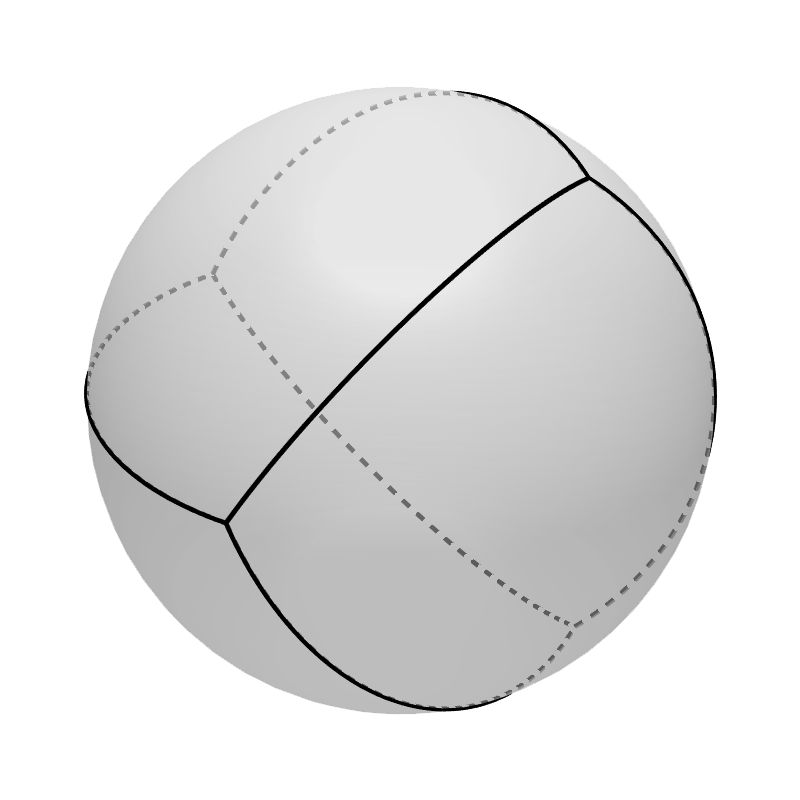
\includegraphics[width=0.4\linewidth]{magdeburg_quarter_sphere.png}
	\caption{}
	\label{fig:Magdeburg季球}
\end{figure}

\subsection{杆上产熵}
均匀细杆的两端分别与恒温热源接触, 其余部分绝热.
因为温度梯度导致的热传导, 杆上存在着热流和熵增.

\mypara
若热流符合 Fourier 热传导定律 $J=-\kappa\nabla T$, 求使得体系 (包括杆和两个热源) 的熵的变化率最小的杆的温度分布.

\mypara
若热流符合线性唯象律 $J=L\nabla\frac1T$, 求使得体系的熵的变化率最小的杆的温度分布, 并说明此时杆达到非平衡定态 (各处的温度不会再随时间改变).

\mypara
若热流符合某种热传导定律 $J=\nabla\varphi\left(T\right)$, 使得体系的熵的变化率最小的杆的温度分布为线性函数 (温度梯度为常数), 求 $\varphi$ 的形式.

提示: 带有固定边界条件 $y\left(a\right)=y_1$, $y\left(b\right)=y_2$ 的变分问题 $\delta\int_a^bL\left(y,y',x\right)=0$ 的解由 Euler--Lagrange 方程 $\frac{\mathrm d}{\mathrm dx}\frac{\partial L}{\partial y'}-\frac{\partial L}{\partial y}=0$ 给出.

\subsection{门外有坏人}
门与地面垂直.
门上高度为 $h$ 处铰接一根长度为 $l>h$ 的质量为 $m$ 的均匀杆.
杆可以在垂直于门的平面内转动.
把杆的自由端放在地上.
杆与地面的静摩擦系数为 $\mu$.

\mypara
若杆足够坚硬, 无论对门施加多大的力都无法推动杆, 求 $\frac hl$ 的范围.

\mypara
若杆不够坚硬, 在上一问的条件下, 对门施加足够大的力可以使杆断裂.
若杆能承受的最大剪切力为 $T$, 求杆的断裂位置的高度.

\subsection{进退两难的死飞}
死飞车是后轮与脚蹬永远处于联动状态的自行车.
图 \ref{fig:自行车结构} 是死飞车的驱动装置简易图.
自行车飞轮半径为 $r_1$, 链轮半径为 $r_2$, 后轮半径为 $R_1$, 曲柄长度为 $R_2$.
规定极轴从飞轮圆心指向链轮圆心.
飞轮圆心到链轮圆心的距离为 $d$.
曲柄和极轴的夹角为 $\theta_2$.
用绳子连接后轮上 $\theta_1$ 处和脚蹬.
求缩短绳子能使自行车前进的条件.
\begin{figure}[h!]
	\centering
	\begin{tikzpicture}
		\draw (0, 0) circle (0.3);
		\draw (0, 0) circle (2.5);
		\draw (5, 0) circle (0.6);
		\draw (-0.09/5, 0.299459513123227) -- (5-0.18/5, 0.598919026246454);
		\draw (-0.09/5, -0.299459513123227) -- (5-0.18/5, -0.598919026246454);
		\draw[double distance = 1mm,line cap=round] (4, 1) -- (6, -1);
		\draw[thick] (1.5, 2) -- (4, 1);
		\draw[dashed] (0, 0) -- (1.5, 2);
		\draw[dashed] (-4, 0) -- (7, 0);
		\node at (0.5, 0.2) {$\theta_1$};
		\node at (5.2, 0.2) {$\theta_2$};
		\node at (-2.3,-1.8) {后轮};
		\node at (-0.5, 0.5) {飞轮};
		\node at (4.7, 0.9) {曲柄};
		\node at (6, 0.3) {链轮};
		\node at (4.1, 1.4) {脚蹬};
	\end{tikzpicture}
	\caption{}
	\label{fig:自行车结构}
\end{figure}

\newpage
\section{参考答案}

\subsection{虹盘天穹}
\mypara
考虑一条被水珠折射的光线.
因为球表面的法线过球心, 所以光线所在平面过球心.
光路如图 \ref{fig:水珠光路图} 所示.

\begin{figure}[h!]
	\centering
	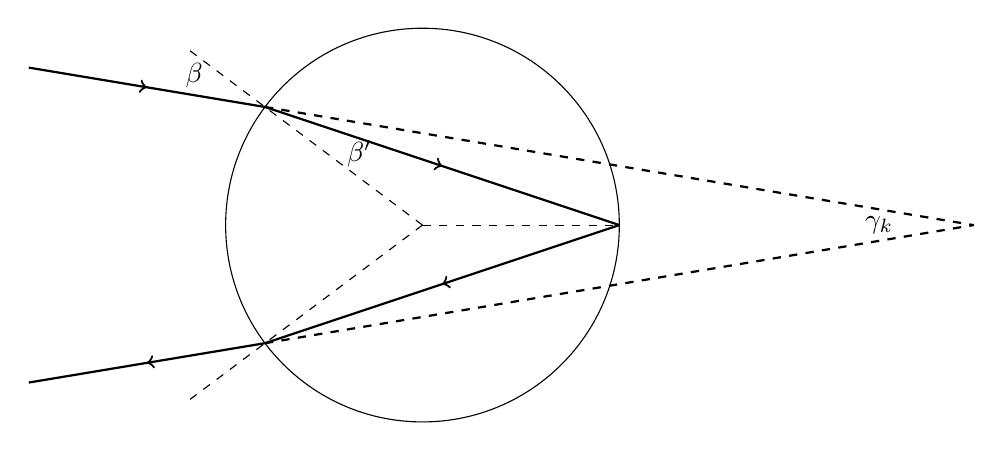
\begin{tikzpicture}
		\draw (0, 0) circle (2.5);
		\begin{scope}[thick,decoration={
				markings,
				mark=at position 0.5 with {\arrow{>}}}
				]
			\draw[postaction={decorate}] (-5,2) -- (-2,1.5);
			\draw[postaction={decorate}] (-2,1.5) -- (2.5,0);
			\draw[postaction={decorate}] (2.5,0) -- (-2,-1.5);
			\draw[postaction={decorate}] (-2,-1.5) -- (-5,-2);
		\end{scope}
		\draw[thick,dashed] (-2,1.5) -- (7,0);
		\draw[thick,dashed] (-2,-1.5) -- (7,0);
		\draw[dashed] (0,0) -- (-3,2.25);
		\draw[dashed] (0,0) -- (-3,-2.25);
		\draw[dashed] (0,0) -- (2.5,0);
		\node at (-2.9,1.9) {$\beta$};
		\node at (-0.8,0.9) {$\beta'$};
		\node at (5.8,0) {$\gamma_k$};
	\end{tikzpicture}
	\caption{}
	\label{fig:水珠光路图}
\end{figure}

设该光线以入射角 $\beta$ 射入水珠, 从而折射角
\begin{equation}
	\beta'=\arcsin\frac{\sin\beta}n.
\end{equation}
每次折射会造成偏转角 $\beta-\beta'$, 每次在水珠内反射会造成偏转角 $\pi-2\beta'$.
总共经历了 $2$ 次折射和 $k-1$ 次反射, 所以总偏转角
\begin{equation}
	\pi-\gamma_k=2\left(\beta-\beta'\right)+\left(k-1\right)\left(\pi-2\beta'\right),
\end{equation}
即入射光线和出射光线的夹角
\begin{equation}
	\gamma_k=\left(2-k\right)\pi-2\beta+2k\arcsin\frac{\sin\beta}n.
	\label{eq:gamma_k}
\end{equation}

设入射光强按 $\beta$ 的分布为 $I\left(\beta\right)\mathrm d\beta$.
显然 $I\left(\beta\right)$ 没有奇点.
但是, 出射光强按 $\gamma_k$ 的分布 $I\left(\beta\right)\frac{\partial\beta}{\partial\gamma_k}\mathrm d\gamma_k$ 可能存在奇点 $\beta=\beta_k$,
即
\begin{equation}
	\left.\frac{\partial\gamma_k}{\partial\beta}\right|_{\beta=\beta_k}=-2+2k\frac{\frac{\cos\beta_k}n}{\sqrt{1-\frac{\sin^2\beta_k}{n^2}}}=0.
\end{equation}
解得
\begin{equation}
	\label{eq:beta_k}
	\beta_k=\arcsin\sqrt{\frac{k^2-n^2}{k^2-1}}.
\end{equation}
将式 \ref{eq:beta_k} 代入式 \ref{eq:gamma_k} 可得
\begin{equation}
	\gamma_k=\left(2-k\right)\pi-2\arcsin\sqrt{\frac{k^2-n^2}{k^2-1}}+2k\arcsin\left(\frac1n\sqrt{\frac{k^2-n^2}{k^2-1}}\right).
	\label{eq:完整的gamma_k}
\end{equation}

在 $\beta=\beta_k$ 处光强发散至无穷大, 因此天球上呈现的曲线就来自于以这一角度入射的光线.

\begin{figure}[h!]
	\centering
	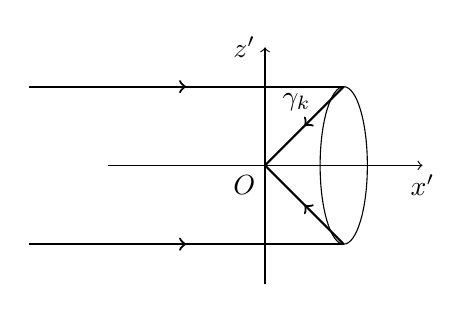
\begin{tikzpicture}
		\begin{scope}[thick,decoration={
				markings,
				mark=at position 0.5 with {\arrow{>}}}
				]
			\draw[postaction={decorate}] (-3,1) -- (1,1);
			\draw[postaction={decorate}] (1,1) -- (0,0);
			\draw[postaction={decorate}] (-3,-1) -- (1,-1);
			\draw[postaction={decorate}] (1,-1) -- (0,0);
		\end{scope}
		\draw (1,0) ellipse (0.3 and 1);
		\node[anchor=north east] at (0,0) {$O$};
		\draw[->] (-2,0) -- (2,0) node [below] {$x'$};
		\draw[->] (0,-1.5) -- (0,1.5) node [left] {$z'$};
		\node at (0.4,0.8) {$\gamma_k$};
	\end{tikzpicture}
	\caption{}
	\label{fig:总光路图}
\end{figure}

即, 若正好背对着太阳看, $k$ 级虹为视角为 $2\gamma_k$ 的圆, 如图 \ref{fig:总光路图} 所示.
若以阳光传播的方向为 $x'$ 轴, 以观察者的位置为原点, 则 $k$ 级虹的曲线方程为
\begin{equation}
	\begin{cases}
		y'^2+z'^2=\sin^2\gamma_k,\\
		x'=\cos\gamma_k.
	\end{cases}
	\label{eq:换系前}
\end{equation}

以向北为 $x$ 轴, 向东为 $y$ 轴 (左手系).
由如图 \ref{fig:换系} 所示的几何关系, 可得 $Oxyz$ 系与 $Ox'y'z'$ 系间的变换关系
\begin{equation}
	\left[\begin{matrix}x'\\y'\\z'\end{matrix}\right]=
	\left[\begin{matrix}\sin\alpha & 0 & -\cos\alpha \\ 0 & 1 & 0 \\ \cos\alpha & 0 & \sin\alpha\end{matrix}\right]
	\left[\begin{matrix}x\\y\\z\end{matrix}\right].
	\label{eq:换系}
\end{equation}

\begin{figure}[h!]
	\centering
	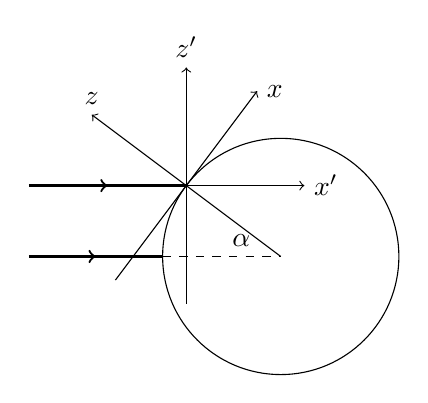
\begin{tikzpicture}
		\draw[->] (1.2,-0.9) circle (1.5);
		\draw[->] (-1.5,0) -- (1.5,0) node [right] {$x'$};
		\draw[->] (0,-1.5) -- (0,1.5) node [above] {$z'$};
		\draw[->] (-0.9,-1.2) -- (0.9,1.2) node [right] {$x$};
		\draw[->] (1.2,-0.9) -- (-1.2,0.9) node [above] {$z$};
		\draw[dashed] (-0.3,-0.9) -- (1.2,-0.9);
		\begin{scope}[thick,decoration={
				markings,
				mark=at position 0.5 with {\arrow{>}}}
				]
			\draw[postaction={decorate}] (-2,0) -- (0,0);
			\draw[postaction={decorate}] (-2,-0.9) -- (-0.3,-0.9);
		\end{scope}
		\node at (0.7,-0.7) {$\alpha$};
	\end{tikzpicture}
	\caption{}
	\label{fig:换系}
\end{figure}

将式 \ref{eq:换系} 代入式 \ref{eq:换系前} 可得新的曲线方程
\begin{equation}
	\begin{cases}
		y^2+\left(x\cos\alpha+z\sin\alpha\right)^2=\sin^2\gamma_k,\\
		x\sin\alpha-z\cos\alpha=\cos\gamma_k.
	\end{cases}
	\label{eq:换系后}
\end{equation}

考虑到地平坐标系的定义, 我们有变换
\begin{equation}
	\left[\begin{matrix}x\\y\\z\end{matrix}\right]=
	\left[\begin{matrix}\cos\theta\cos\varphi \\ \cos\theta\sin\varphi \\ \sin\theta\end{matrix}\right].
	\label{eq:地平坐标系}
\end{equation}
将式 \ref{eq:地平坐标系} 代入式 \ref{eq:换系后} 可得地平坐标系中 $k$ 级虹的曲线方程
\begin{equation}
	\begin{cases}
		\cos^2\theta\sin^2\varphi+\left(\cos\theta\cos\varphi\cos\alpha+\sin\theta\sin\alpha\right)^2=\sin^2\gamma_k,\\
		\cos\theta\cos\varphi\sin\alpha-\sin\theta\cos\alpha=\cos\gamma_k.
	\end{cases}
	\label{eq:地平坐标系冗余曲线方程}
\end{equation}
但是注意到式 \ref{eq:地平坐标系冗余曲线方程} 中的两式可以相互推出 (这源于球坐标自带球面约束而导致的坐标数量的减少), 实际上可以简化为一个式子
\begin{equation}
	\cos\theta\cos\varphi\sin\alpha-\sin\theta\cos\alpha=\cos\gamma_k.
	\label{eq:地平坐标系曲线方程}
\end{equation}

式 \ref{eq:地平坐标系曲线方程} 和式 \ref{eq:完整的gamma_k} 给出了答案.

\mypara
需要求出式 \ref{eq:地平坐标系曲线方程} 所描述的曲线上使得 $\theta>0$ (即在天顶上) 的部分 (圆弧) 的长度占整条曲线 (圆) 的比例 $r$.
为此, 将
\begin{equation}
	\theta=0
	\label{eq:地平线}
\end{equation}
代入式 \ref{eq:地平坐标系曲线方程}, 得
\begin{equation}
	\cos\varphi=\frac{\cos\gamma_k}{\sin\alpha}.
	\label{eq:地平线上的phi满足的方程}
\end{equation}

\begin{enumerate}

	\item
	对于 $\left|\sin\alpha\right|<\left|\cos\gamma_k\right|$, 式 \ref{eq:地平线上的phi满足的方程} 无解.
	从而 $k$ 级虹与地平线没有交点, 即人们能看到完整的圆形虹 ($r=1$)或完全看不到虹 ($r=0$).
	经过简单分析可得, 这种情形下, 对于 $\cos\gamma_k>0$, 有 $r=0$; 对于 $\cos\gamma_k<0$, 有 $r=1$.

	\item
	对于 $\left|\sin\alpha\right|>\left|\cos\gamma_k\right|$, 式 \ref{eq:地平线上的phi满足的方程} 的解 (在模 $2\pi$ 下) 为
	\begin{equation}
		\varphi=\pm\arccos\frac{\cos\gamma_k}{\sin\alpha}.
		\label{eq:地平线上的phi}
	\end{equation}
	将式 \ref{eq:地平线} 和式 \ref{eq:地平线上的phi} 代入式 \ref{eq:地平坐标系} 可得 $k$ 级虹与地平线的交点为
	$\left(\frac{\cos\gamma_k}{\sin\alpha},\pm\sqrt{1-\frac{\cos^2\gamma_k}{\sin^2\alpha}},0\right)$.
	即, $k$ 级虹被地平线所截弦所对的圆心角为
	\begin{equation}
		\psi=2\arcsin\frac{\sqrt{1-\frac{\cos^2\gamma_k}{\sin^2\alpha}}}{\left|\sin\gamma_k\right|}.
	\end{equation}
	经过简单分析可得, 在这种情况下, 对于 $\cos\gamma_k>0$, 有 $r=\frac\psi{2\pi}$; 对于 $\cos\gamma_k<0$, 有 $r=1-\frac\psi{2\pi}$.

\end{enumerate}

注意到 $\Delta n$ 为小量, 故由式 \ref{eq:完整的gamma_k} 有
\begin{equation}
	\Delta\gamma_k=\frac{\partial\gamma_k}{\partial n}\Delta n=-\frac{2\Delta n}n\sqrt{\frac{k^2-n^2}{n^2-1}}.
	\label{eq:delta gamma_k}
\end{equation}
从而利用式 \ref{eq:delta gamma_k} 易得答案
\begin{equation}
	\Omega=r\cdot2\pi\left|\sin\gamma_k\cdot\Delta\gamma_k\right|=4\pi r\left|\sin\gamma_k\right|\frac{\Delta n}n\sqrt{\frac{k^2-n^2}{n^2-1}},
\end{equation}
其中
\begin{equation}
	r=
	\begin{cases}
		0, & \left|\sin\alpha\right|<\left|\cos\gamma_k\right|,\cos\gamma_k>0\\
		1, & \left|\sin\alpha\right|<\left|\cos\gamma_k\right|,\cos\gamma_k<0\\
		\frac1\pi\arcsin\frac{\sqrt{1-\frac{\cos^2\gamma_k}{\sin^2\alpha}}}{\left|\sin\gamma_k\right|}, & \left|\sin\alpha\right|>\left|\cos\gamma_k\right|,\cos\gamma_k>0\\
		1-\frac1\pi\arcsin\frac{\sqrt{1-\frac{\cos^2\gamma_k}{\sin^2\alpha}}}{\left|\sin\gamma_k\right|}, & \left|\sin\alpha\right|>\left|\cos\gamma_k\right|,\cos\gamma_k<0
	\end{cases}
\end{equation}
$\gamma_k$ 由式 \ref{eq:完整的gamma_k} 给出.

\mypara
显然 $k$ 级虹上具有最大高度角的点的方位角与太阳的方位角相同或者相差 $\pi$, 因此 $k$ 级虹上具有最大高度角的点的方位角的变化率等同于太阳的方位角的变化率.

在春分日 $\frac{\eta+\pi}{2\pi}\cdot 24$ 时 (24 小时制) 时刻, 以阳光传播的方向为 $x'$ 轴, 以平行于地球自转轴向北为 $z'$ 轴, 建立 $Ox'y'z'$ 左手系.
以地平线为 $xy$ 平面, 以正北为 $x$ 轴, 以正东为 $y$ 轴, 建立 $Oxyz$ 左手系.
由几何关系可知, 在 $Ox'y'z'$ 坐标系中, $y$ 方向的单位矢量为
\begin{equation}
	\mathbf y=\left[\begin{matrix}\sin\eta \\ \cos\eta \\ 0\end{matrix}\right],
\end{equation}
$x$ 方向的单位矢量为
\begin{equation}
	\mathbf x=\left[\begin{matrix}\sin\alpha\cos\eta \\ -\sin\alpha\sin\eta \\ \cos\alpha\end{matrix}\right].
\end{equation}
从而可得 $x'$ 方向的单位矢量在 $y$ 方向的分量为 $\sin\eta$, 而其在 $x$ 方向的分量为 $\sin\alpha\cos\eta$.
这两个分量的比值为太阳的方位角的正切值, 即
\begin{equation}
	\varphi^*=\arctan\frac{\sin\eta}{\sin\alpha\cos\eta}.
	\label{eq:太阳的方位角}
\end{equation}
将其对时间求导并代入 $\eta=0$, 考虑到 $\dot\eta=\omega$, 有
\begin{equation}
	\left.\dot\varphi^*\right|_{\eta=0}=\frac\omega{\sin\alpha}.
\end{equation}
这一结果意味着在北半球上看到的南方的 $k$ 级虹和在南半球上看到的北方的 $k$ 级虹会向西移动, 而在北半球上看到的北方的 $k$ 级虹和在南半球上看到的南方的 $k$ 级虹会向东移动.

\subsection{Magdeburg 季球}

\subsection{杆上产熵}
设 $t$ 时刻杆在 $x\in\left[a,b\right]$ 处的温度为 $T\left(t,x\right)$,
熵线密度为 $s\left(t,x\right)$,
单位时间内通过 $x$ 处的热量 (即 $x$ 处的热流) 为 $J\left(t,x\right)$.
两个恒温热源的温度分别为
\begin{equation}
T\left(t,a\right)=T_a,\qquad T\left(t,b\right)=T_b.
\label{eq:变分边界条件}
\end{equation}

取杆上的线微元 $\left[x,x+\mathrm dx\right]$.
在 $\mathrm dt$ 时间内, 在 $x$ 处有 $J\left(t,x\right)\mathrm dt$ 的热量流入该线微元,
在 $x+\mathrm dx$ 处有 $J\left(t,x+\mathrm dx\right)\mathrm dt$ 的热量流出该线微元,
从而 $t+\mathrm dt$ 时刻该线微元获得熵增
\begin{equation}
\frac{J\left(t,x\right)\mathrm dt-J\left(t,x+\mathrm dx\right)\mathrm dt}{T}=-\frac1T\frac{\partial J}{\partial x}\mathrm dx\mathrm dt,
\end{equation}
即
\begin{equation}
\frac{\partial s}{\partial t}=-\frac1T\frac{\partial J}{\partial x}.
\label{eq:熵线密度的变化速率}
\end{equation}

将式 \ref{eq:熵线密度的变化速率} 对 $x$ 积分, 可得杆的熵产
\begin{equation}
\frac{\mathrm dS_0}{\mathrm dt}=\int_a^b\frac{\partial s}{\partial t}\mathrm dx=\int_a^b-\frac1T\frac{\partial J}{\partial x}\mathrm dx.
\label{eq:杆的熵产前}
\end{equation}
对式 \ref{eq:杆的熵产前} 右边应用分部积分可得
\begin{equation}
\frac{\mathrm dS_0}{\mathrm dt}=-\frac{J\left(t,b\right)}{T_b}+\frac{J\left(t,a\right)}{T_a}+\int_a^bJ\frac{\partial\frac1T}{\partial x}\mathrm dx.
\label{eq:杆的熵产}
\end{equation}

另一方面, 显然, 两个恒温热源的熵产分别为
\begin{equation}
\frac{\mathrm dS_a}{\mathrm dt}=-\frac{J\left(t,a\right)}{T_a},\qquad
\frac{\mathrm dS_b}{\mathrm dt}=\frac{J\left(t,b\right)}{T_b}.
\label{eq:热源的熵产}
\end{equation}
将式 \ref{eq:杆的熵产} 与式 \ref{eq:热源的熵产} 相加, 得到整个体系的熵产
\begin{equation}
\frac{\mathrm dS}{\mathrm dt}=\int_a^bJ\frac{\partial\frac1T}{\partial x}\mathrm dx=\int_a^b-\frac{J}{T^2}\frac{\partial T}{\partial x}\mathrm dx.
\label{eq:整个体系的熵产}
\end{equation}

令
\begin{equation}
\mathcal L\left(T,T',x\right)=-J\left(T,T'\right)\frac{T'}{T^2},
\label{eq:lagrangian}
\end{equation}
其中 $T'=\nabla T=\frac{\partial T}{\partial x}$.
注意, 这里 $J\left(T,T'\right)$ 与前文中的 $J\left(t,x\right)$ 虽然是同一个物理量, 但具有不同的意义.
$J\left(T,T'\right)$ 表征了与热传导有关的物理定律, Fourier 热传导定律是它的一个例子.
显然, 由时空平移不变性, 当作为物理定律时, $J$ 不应与 $t,x$ 有关.

此时最小化熵产的问题转化为变分问题
\begin{equation}
\delta\int_a^b\mathcal L\left(T,T',x\right)\mathrm dx=0,
\end{equation}
其中在变分过程中有固定的边界条件式 \ref{eq:变分边界条件}.
写出 Euler--Lagrange 方程
\begin{equation}
\frac{\partial}{\partial x}\frac{\partial\mathcal L}{\partial T'}-\frac{\partial\mathcal L}{\partial T}=0
\label{eq:EL方程}
\end{equation}
(这里的 $\frac{\partial}{\partial x}$ 要求将 $T,T'$ 看作是依赖于 $x$ 的, 但 $t$ 是不依赖于 $x$ 的).

为了利用式 \ref{eq:EL方程}, 根据式 \ref{eq:lagrangian} 写出 $L$ 的偏导数
\begin{equation}
\frac{\partial\mathcal L}{\partial T}=-T'\left(\frac{\partial J}{\partial T}\frac1{T^2}-\frac{2J}{T^3}\right),
\qquad\frac{\partial\mathcal L}{\partial T'}=-\frac{1}{T^2}\left(\frac{\partial J}{\partial T'}T'+J\right),
\qquad\frac{\partial\mathcal L}{\partial x}=0.
\label{eq:lagrangian的偏导数}
\end{equation}
将式 \ref{eq:lagrangian的偏导数} 代入式 \ref{eq:EL方程} 可得
\begin{equation}
\frac{\partial}{\partial x}\left(-\frac{1}{T^2}\left(\frac{\partial J}{\partial T'}T'+J\right)\right)+T'\left(\frac{\partial J}{\partial T}\frac1{T^2}-\frac{2J}{T^3}\right)=0.
\label{eq:一般的J的EL方程}
\end{equation}

\mypara
将 Fourier 热传导定律 $J\left(T,T'\right)=-\kappa T'$ 代入式 \ref{eq:一般的J的EL方程} 可得
\begin{equation}
	\frac{\partial}{\partial x}\frac{2\kappa T'}{T^2}+\frac{2\kappa T'^2}{T^3}=0.
	\label{eq:Fourier热传导定律的EL方程}
\end{equation}
由式 \ref{eq:Fourier热传导定律的EL方程} 可得关于 $T\left(x\right)$ 的常微分方程
\begin{equation}
	T''=\frac{T'^2}{T}.
\end{equation}
将 $T''$ 写成 $T'\frac{\mathrm dT'}{\mathrm dT}$, 进行两次分离变量和积分, 由边界条件式 \ref{eq:变分边界条件} 确定积分常数.
最终可得温度分布
\begin{equation}
	T=T_a\left(\frac{T_b}{T_a}\right)^{\frac{x-a}{b-a}}.
\end{equation}

\mypara
将线性唯象律 $J\left(T,T'\right)=L\nabla\frac1T=-\frac{LT'}{T^2}$ 代入式 \ref{eq:一般的J的EL方程}.
经过与上一问类似的操作, 最终可得温度分布
\begin{equation}
	T=\frac{T_a}{1-\frac{x-a}{b-a}\left(1-\frac{T_a}{T_b}\right)}.
\end{equation}
显然, 该温度分布能使得温度倒数的梯度在杆上处处相等.
由于线性唯象律给出热流与温度倒数的梯度成正比, 该温度分布能使得杆上的热流处处相等.
从而热流的散度为零, 热量无法积累使得内能密度改变, 体系达到非平衡定态.

\mypara
将 $J\left(T,T'\right)=\nabla\varphi\left(T\right)=\varphi'\left(T\right)T'$ 代入式 \ref{eq:lagrangian} 可得
\begin{equation}
	\mathcal L=-\frac{\varphi'\left(T\right)T'^2}{T^2}.
	\label{eq:线性温度分布的lagrangian}
\end{equation}
从而
\begin{align}
	\frac{\partial}{\partial x}\frac{\partial\mathcal L}{\partial T'}
	=\frac{\partial}{\partial x}\left(-\frac{2\varphi'\left(T\right)T'}{T^2}\right)=-2T'^2\frac{\partial}{\partial T}\frac{\varphi'\left(T\right)}{T^2}-2T''\frac{\varphi'\left(T\right)}{T^2},
	\label{eq:线性温度分布的EL方程第一项}
\end{align}
\begin{equation}
	\frac{\partial\mathcal L}{\partial T}=-T'^2\frac{\partial}{\partial T}\frac{\varphi'\left(T\right)}{T^2}.
	\label{eq:线性温度分布的EL方程第二项}
\end{equation}

将式 \ref{eq:线性温度分布的EL方程第一项} 和式 \ref{eq:线性温度分布的EL方程第二项} 代入 \ref{eq:EL方程} 后整理可得
\begin{equation}
	\frac{\mathrm d}{\mathrm dT}\ln\frac{\varphi'\left(T\right)}{T^2}=-\frac{2T''}{T'^2}.
\end{equation}
对于温度梯度处处为常数的温度分布, $T''=0$.
从而 $\frac{\varphi'\left(T\right)}{T^2}$ 为常数.
从而应有
\begin{equation}
	\varphi\left(T\right)=-kT^3+C,
\end{equation}
其中 $k$ 和 $C$ 为积分常量 (答案中不包含 $C$ 项也算对).
注意到最终的熵产是最小值而不是最大值, 应有 $k>0$.

\subsection{门外有坏人}
\mypara
设杆与地面间的弹力为 $N$, 静摩擦力为 $f$.

如图 \ref{fig:杆受力分析}, 对杆进行受力分析.

\begin{figure}
	\centering
	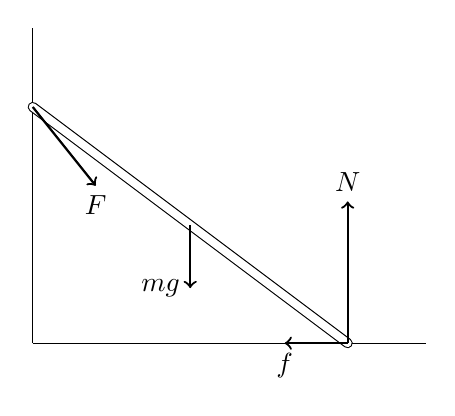
\begin{tikzpicture}
		\draw (0, 0) -- (0, 4);
		\draw (0, 0) -- (5, 0);
		\draw[double distance = 1mm,line cap=round] (0, 3) -- (4, 0);
		\draw[thick,->] (0, 3) -- (0.8, 2) node [anchor=north] {$F$};
		\draw[thick,->] (2, 1.5) -- (2, 0.7) node [anchor=east] {$mg$};
		\draw[thick,->] (4, 0) -- (4, 1.8) node [anchor=south] {$N$};
		\draw[thick,->] (4, 0) -- (3.2, 0) node [anchor=north] {$f$};
	\end{tikzpicture}
	\caption{}
	\label{fig:杆受力分析}
\end{figure}

对铰链处总力矩为零, 可得
\begin{equation}
	fh+mg\frac{\sqrt{l^2-h^2}}2-N\sqrt{l^2-h^2}=0.
\end{equation}
整理得
\begin{equation}
	\frac fN=\left(1-\frac{mg}{2N}\right)\sqrt{\frac{l^2}{h^2}-1}<\sqrt{\frac{l^2}{h^2}-1}.
\end{equation}
为保证不滑动, 对于任意的 $N$, $\frac fN$ 应恒小于 $\mu$.
从而
\begin{equation}
	\mu\ge\sqrt{\frac{l^2}{h^2}-1},
\end{equation}
即 $\frac hl\in\left[\frac1{\sqrt{1+\mu^2}},1\right)$.

\mypara


\subsection{进退两难的死飞}
由齿轮-链条约束, 有
\begin{equation}
	r_1\mathrm d\theta_1=r_2\mathrm d\theta_2=\mathrm dx,
	\label{eq:齿轮-链条约束}
\end{equation}
其中 $\mathrm dx$ 是人为定义的微元.
$\mathrm dx<0$ 表征自行车前进, $\mathrm dx>0$ 表征自行车后退.

由几何关系易得连接后轮和脚蹬的绳子的长度的平方
\begin{equation}
	l^2=\left(R_2\cos\theta_2-R_1\cos\theta_1+d\right)^2+\left(R_2\sin\theta_2-R_1\sin\theta_1\right)^2.
	\label{eq:绳子长度}
\end{equation}
对式 \ref{eq:绳子长度} 两边取微分, 得
\begin{equation}
\begin{split}
	2l\mathrm dl
	=2&\left(R_2\cos\theta_2-R_1\cos\theta_1+d\right)\left(-R_2\sin\theta_2\mathrm d\theta_2+R_1\sin\theta_1\mathrm d\theta_1\right)+\\
	2&\left(R_2\sin\theta_2-R_1\sin\theta_1\right)\left(R_2\cos\theta_2\mathrm d\theta_2-R_1\cos\theta_1\mathrm d\theta_1\right).
\end{split}
\end{equation}
全部展开并整理, 再利用式 \ref{eq:齿轮-链条约束} 可得
\begin{equation}
	l\mathrm dl=R_1R_2\sin\left(\theta_2-\theta_1\right)\left(\frac1{r_2}-\frac1{r_1}\right)\mathrm dx-d\left(\frac{R_2\sin\theta_2}{r_2}-\frac{R_1\sin\theta_1}{r_1}\right)\mathrm dx.
\end{equation}
缩短绳子使得自行车前进的条件是 $\mathrm dl/\mathrm dx>0$.
从而
\begin{equation}
	R_1R_2\left(r_1-r_2\right)\sin\left(\theta_2-\theta_1\right)>d\left(r_1R_2\sin\theta_2-r_2R_1\sin\theta_1\right).
\end{equation}

\end{document}
